\chapter{The ATLAS Detector} \label{chap:atlas}

Given the immense energies available at the LHC, and the veritable zoo of
paricles we are trying to detect, we require a general-purpose experiment in
order to fully exploit the full range of physics opportunities provided.  Two
international collaborations rose to this challenge, the CMS (Compact Muon
Solenoid) and ATLAS (A Toroidal LHC ApparatuS) experiments.  While both have
similar physics goals and each of them strengths and weaknesses, this
dissertation will focus on the ATLAS experiment and the intricacies of its three
sub-detectors and two massive magnet systems depicted in
\Cref{fig:atlas_cutaway}.

\begin{figure}[!htbp]
  \begin{center}
    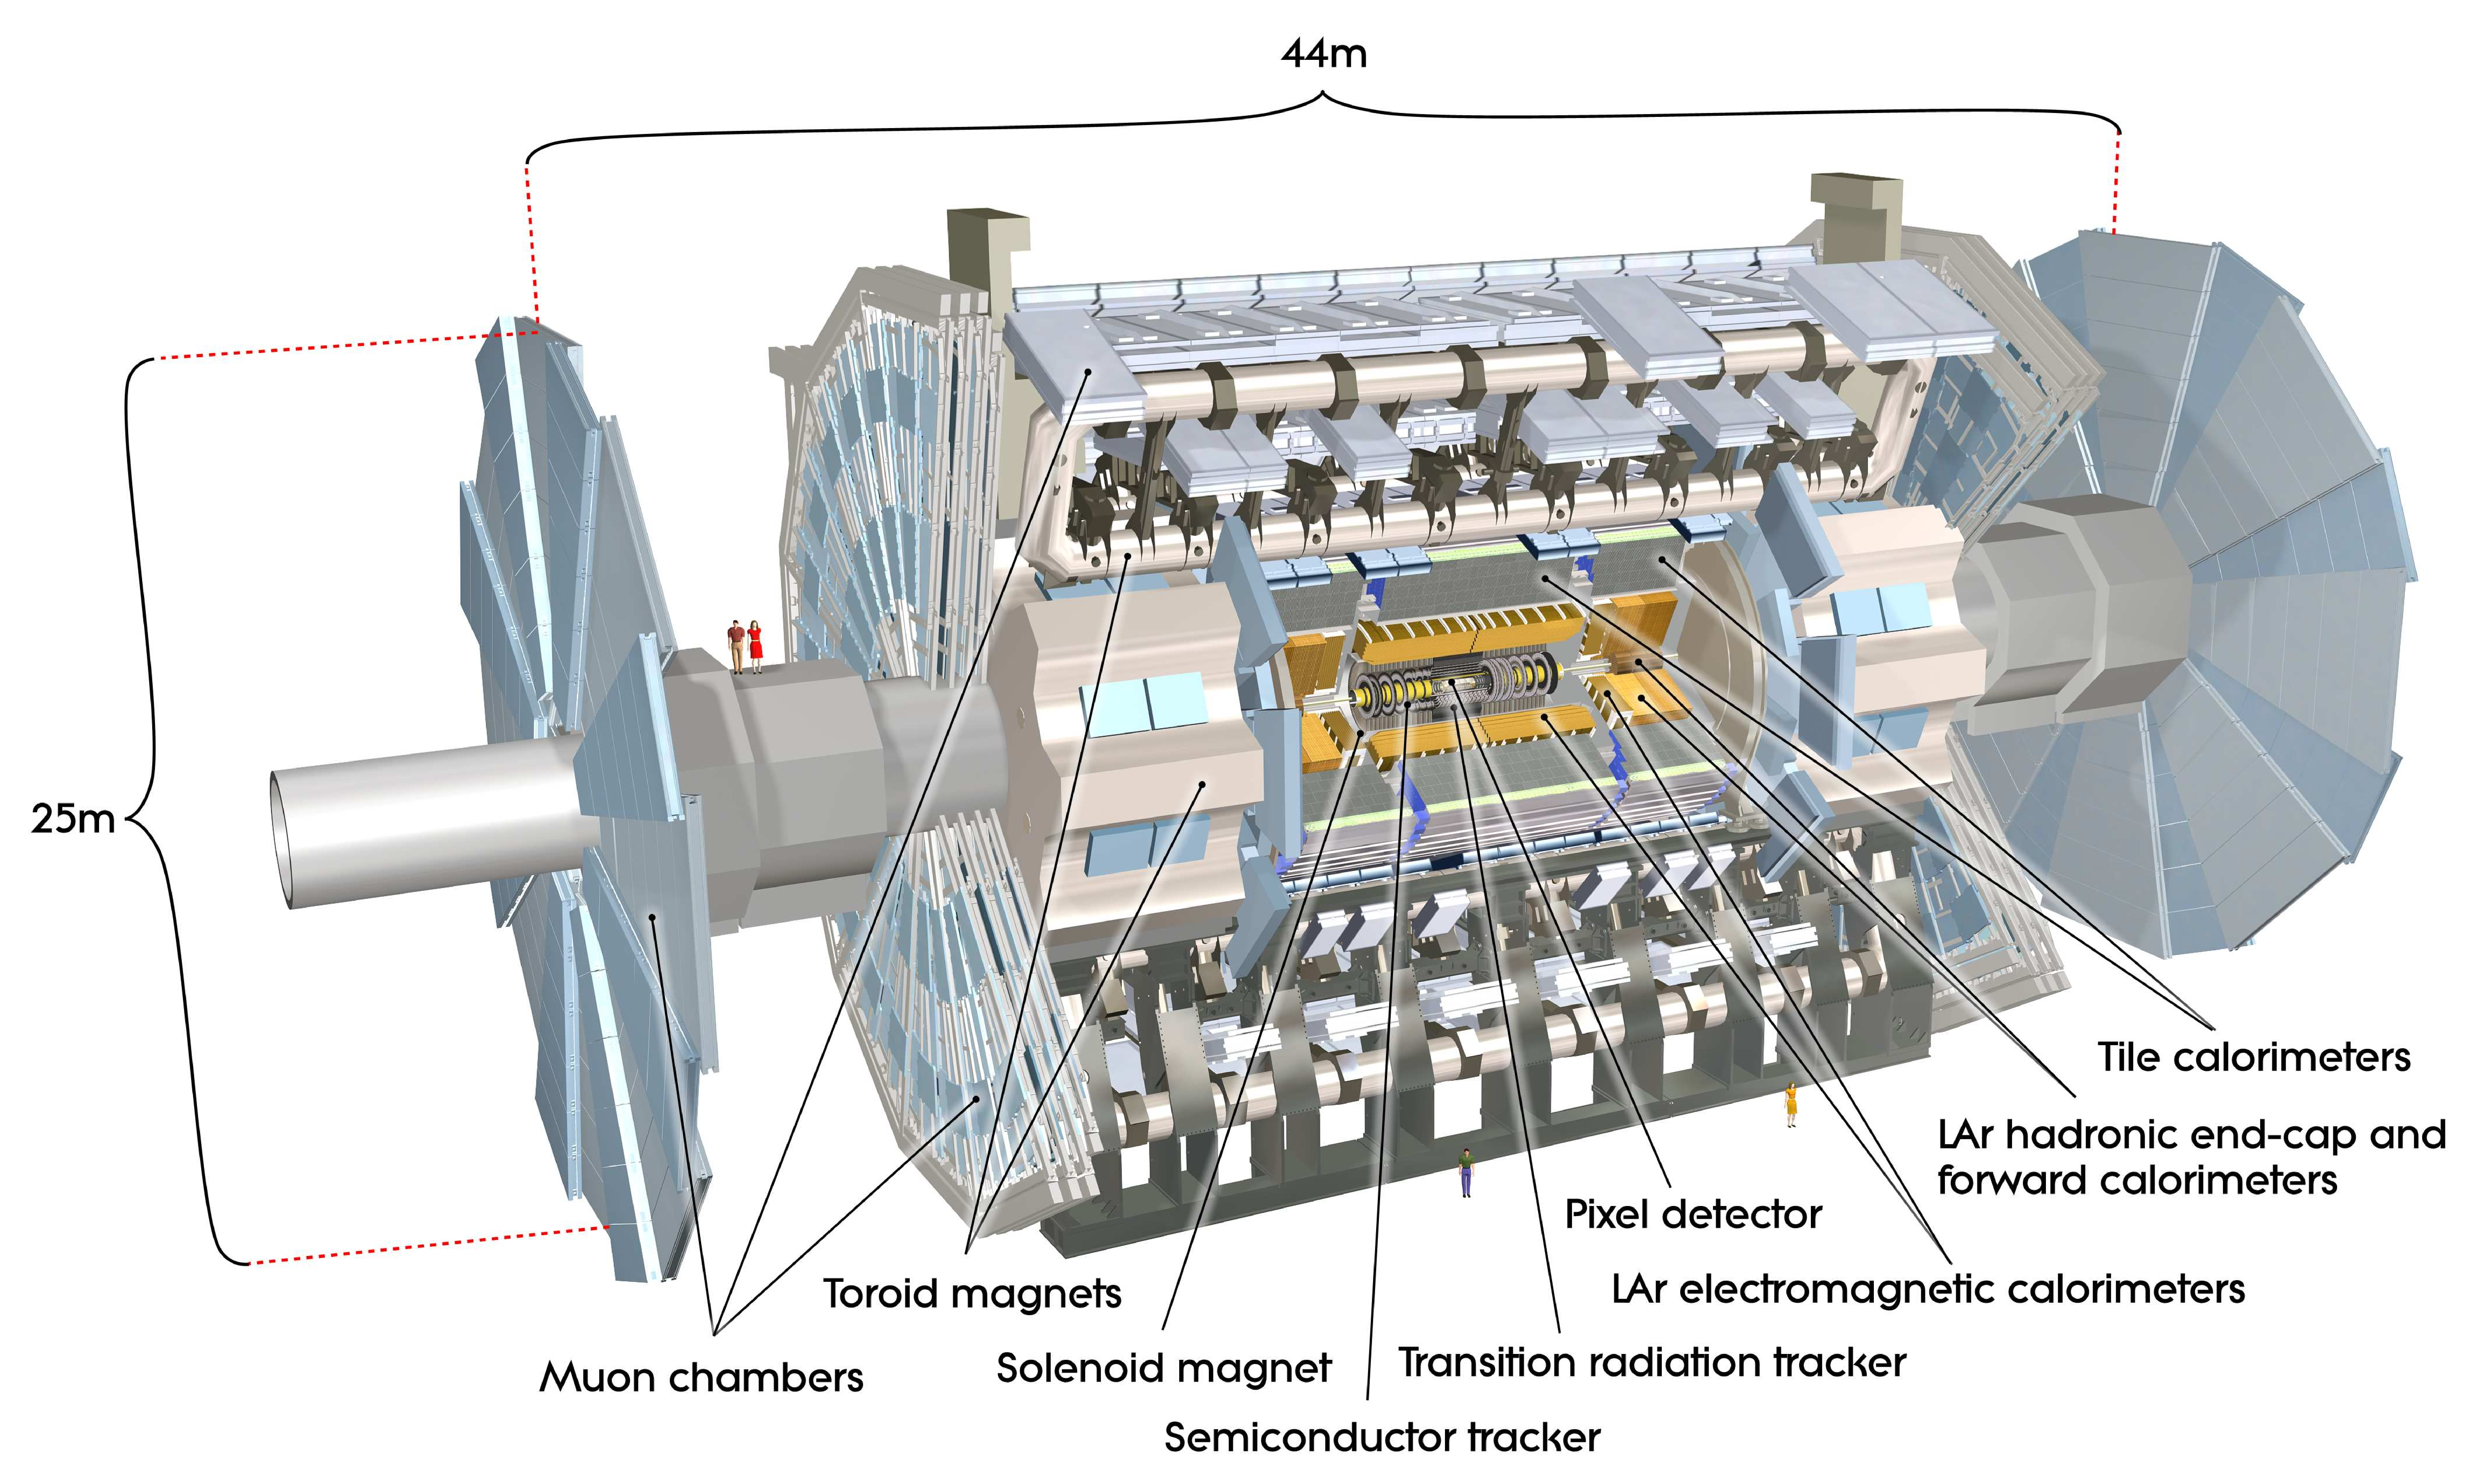
\includegraphics[width=0.9\linewidth]{figures/atlas/atlas_cutaway.pdf}
    \caption{ \cite{PERF-2007-01} Here we see a cut-away side view of the ATLAS
detector with the major components labeled.  Note that within each of these
labeled components there may exist multiple different detector technologies.
For scale two people in red are shown standing between the disk muon chambers on the
left side of the figure. }
    \label{fig:atlas_cutaway}
  \end{center}
\end{figure}

Originally proposed in 1994, the ATLAS detector was completed in 2008. On
July 4th, 2012 in a joint announcement the ATLAS and CMS experiments presented
the discovery of the long predicted Higgs Boson.  The ATLAS collaboration now boasts
over 3000 physicists from 175 institutions spread across 38 countries and
continues to probe the limits of the Standard Model in pursuit of answers to
some of humanity's deepest questions.

Located approximately 100 meters underground in a vast excavated chamber, the
ATLAS detector rests its 7000 metric tons on a bed of concrete-reinforced
steel.  Out of it flows the signals from 100 million electronic channels
through a zip-tied mass of 3000+ kilometers of cabling.  At its very center is
one of the four interaction points of the LHC, specifically Point 1, where the
two counter circulating proton beams are shaped and then brought together by a
series of magnets.  The energetic particles resulting from this collision then
fly out in all directions into the bulk of the ATLAS detector.

The first sub-system they meet is the Inner Detector (ID) and its many layers of
strip and pixel silcon detectors along with a transition radiation gaseous wire
detector, all bathed in the 2T mangnetic field from the surrounding superconducting
solenoidal magnet.  This system exploits the ionization of charged particles to
track their curved trajectory through the magnetic field.  This curvature gives
us charge information, a momentum measurement, and precisely-located 3D vertices
crucial to the identification of the secondary vertices of a B-hadron decay. 

Outside of the solenoid the particles encounter the Electromagnetic and then
the Hadronic sampling calorimeters. Here, layers of scintillator and high
radiation length materials are implemented to measure the energy of electrons,
photons, and hadrons. As the goal is to completely absorb the energy of all
outgoing particles the calorimeter has a nearly $4\pi$ solid angle coverage.

Finally we have the muon system surrounding the calorimeter and equipped with
its own toroidal magnet system.  Here the charged muon bends in the magnetic
field while leaving a trail of ionization in the Muon Spectrometer before
exiting the detector completely.  Neutrinos are the only other Standard Model
particle that leave the detector, however they do so without detection.  A
depiction of the various particle interactions with the different detector
sub-systems can be seen in \Cref{fig:detector_interactions}

In the following sections I will explain our chosen coordinate system and give 
a more detailed review of these three detector sub-systems.

\begin{figure}[!htbp]
  \begin{center}
    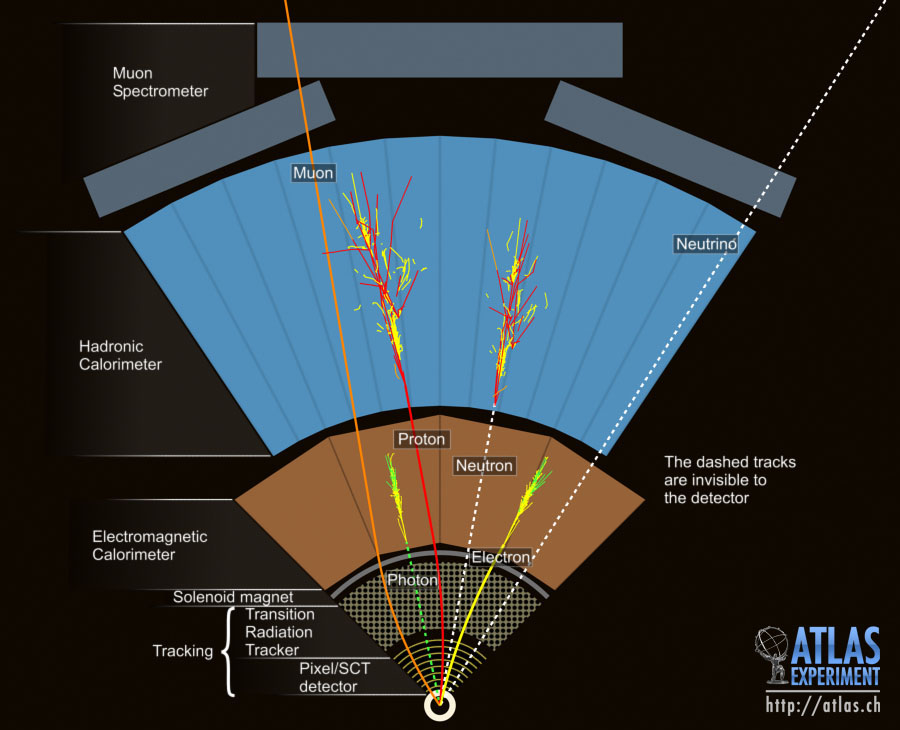
\includegraphics[width=0.9\linewidth]{figures/atlas/detector_interactions}
    \caption{This slice of the ATLAS detector depicts how different particles
interact with each component of the detector it crosses.  A dashed line
indicates no interaction while a solid line indicates interaction. Electrons
(yellow/green) and charged hadrons (red) interact with the tracker and curve in
the solenoid's magnetic field.  Electrons and photons (yellow/green) are
absorbed by the Electromagnetic calorimeter.  All hadrons (red/yellow) are
absorbed by the Hadronic calorimeter. The muons (orange) curve in both the
solenoid and toroid magnetic fields before exiting the detector. Finally, the
neutrinos (white) pass through the entire detector without interacting.  }
    \label{fig:detector_interactions}
  \end{center}
\end{figure}

\section{ATLAS Coordinate System} \label{sec:atlas:coordinates}

Choosing the nominal interaction point as the origin, ATLAS defines a right-handed
coordinate system where the positive $x$-axis points towards the center of the
LHC ring, the positive $y$-axis points upwards, and the positive $z$-axis is
defined by the counter-clockwise circulating beam direction as viewed from
above, as shown in \Cref{fig:atlas_geometry} \cite{PERF-2007-01}.  
 
\begin{figure}[!htbp]
  \begin{center}
    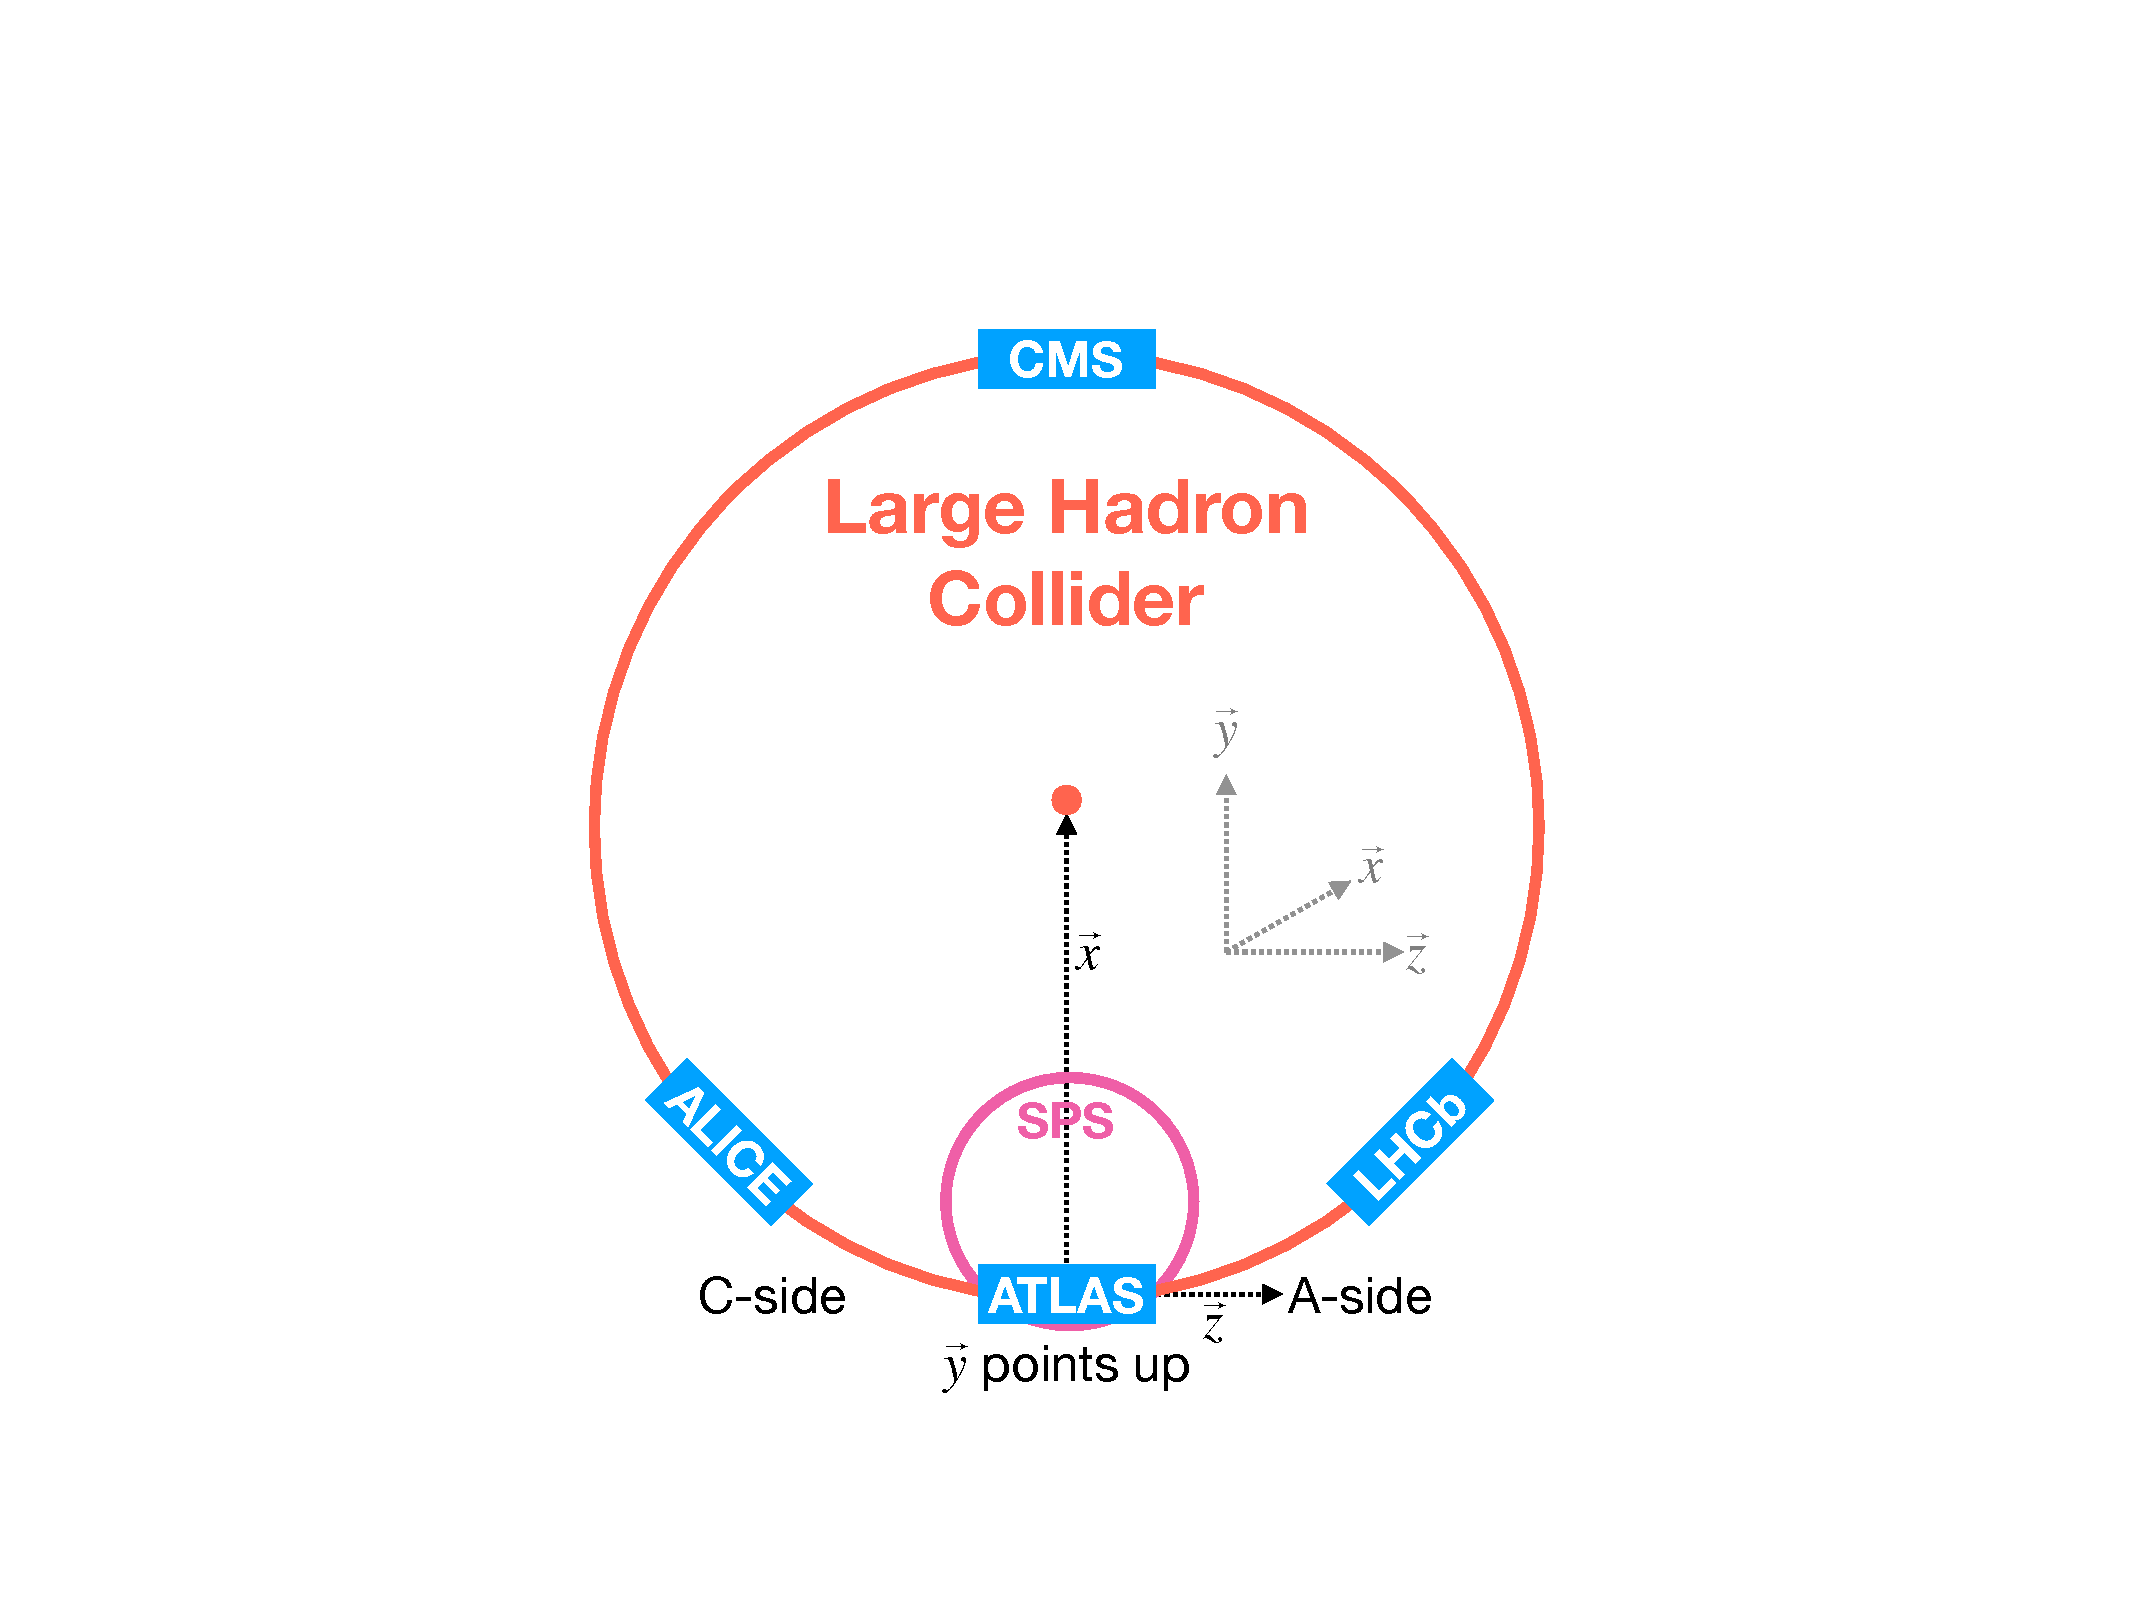
\includegraphics[width=0.7\linewidth]{figures/atlas/atlas_geometry}
    \caption{ The standard Cartesian coordinate system is shown with its origin at
the ATLAS interaction point, the positive $x$-axis towards the center of the
LHC, the positive $y$-axis pointing upwards, and the positive $z$-axis pointing
along the beamline \cite{Feickert:2690521}.}
    \label{fig:atlas_geometry}
  \end{center}
\end{figure}

Using these coordinates the physical momentum of the objects measured is
defined as $\vec{p} = (\pt,p_z)$ with \pt being the momentum of the object in
the transverse plane and $p_z$ the momentum along the beam axis. Considering
the cylindrical symmetry of ATLAS it is desirable to define the polar angle
$\theta$ from the beam axis with the $r$-$\phi$ plane being perpendicular to
that axis.  The radial distance is defined as $r = \sqrt{x^2+y^2}$ and the
azimuthal angle is defined with $\phi = 0$ corresponding to the $x$-axis.

The initial state of a collision is inevitably boosted in the $z$-axis, however
there is no way to measure this boost so it is important to define our
geometric quantities to be invariant under these boosts. In the high energy
regime, the pseudorapidity 

\begin{equation}
 \eta = -\ln \tan \left( \frac{\theta}{2} \right)
\end{equation}

is a good approximation of the rapidity ($y$) of a particle --- a measurement of
the velocity of a particle longitudinal to the beam axis ($z$-axis)

\begin{equation}
y = \frac{1}{2} \ln \left( \frac{E + p_{z}}{E - p_{z}} \right)
\end{equation}

where $E$ is the energy of the particle and $p_{z}$ is defined above.
Differences in rapidity ($\Delta\eta$) are Lorentz invariant under boosts along
the $z$-axis.  However, pseudorapidity is preferred as it is an entirely
geometric quantity independent of particle energy. \Cref{fig:pseudorapidity}
gives a sense of the distribution of $\eta$ in the $y$-$z$ plane. Since $\phi$
is defined in the $x$-$y$ plane, differences in the azimuthal angle
($\Delta\phi$) are also invariant under Lorentz boosts along the $z$-axis.
This allows for the definition of a Lorentz invariant angular separation

\begin{equation}
 \DeltaRdef \,
\end{equation}

between objects in the detector.

\begin{figure}[!htbp]
  \begin{center}
    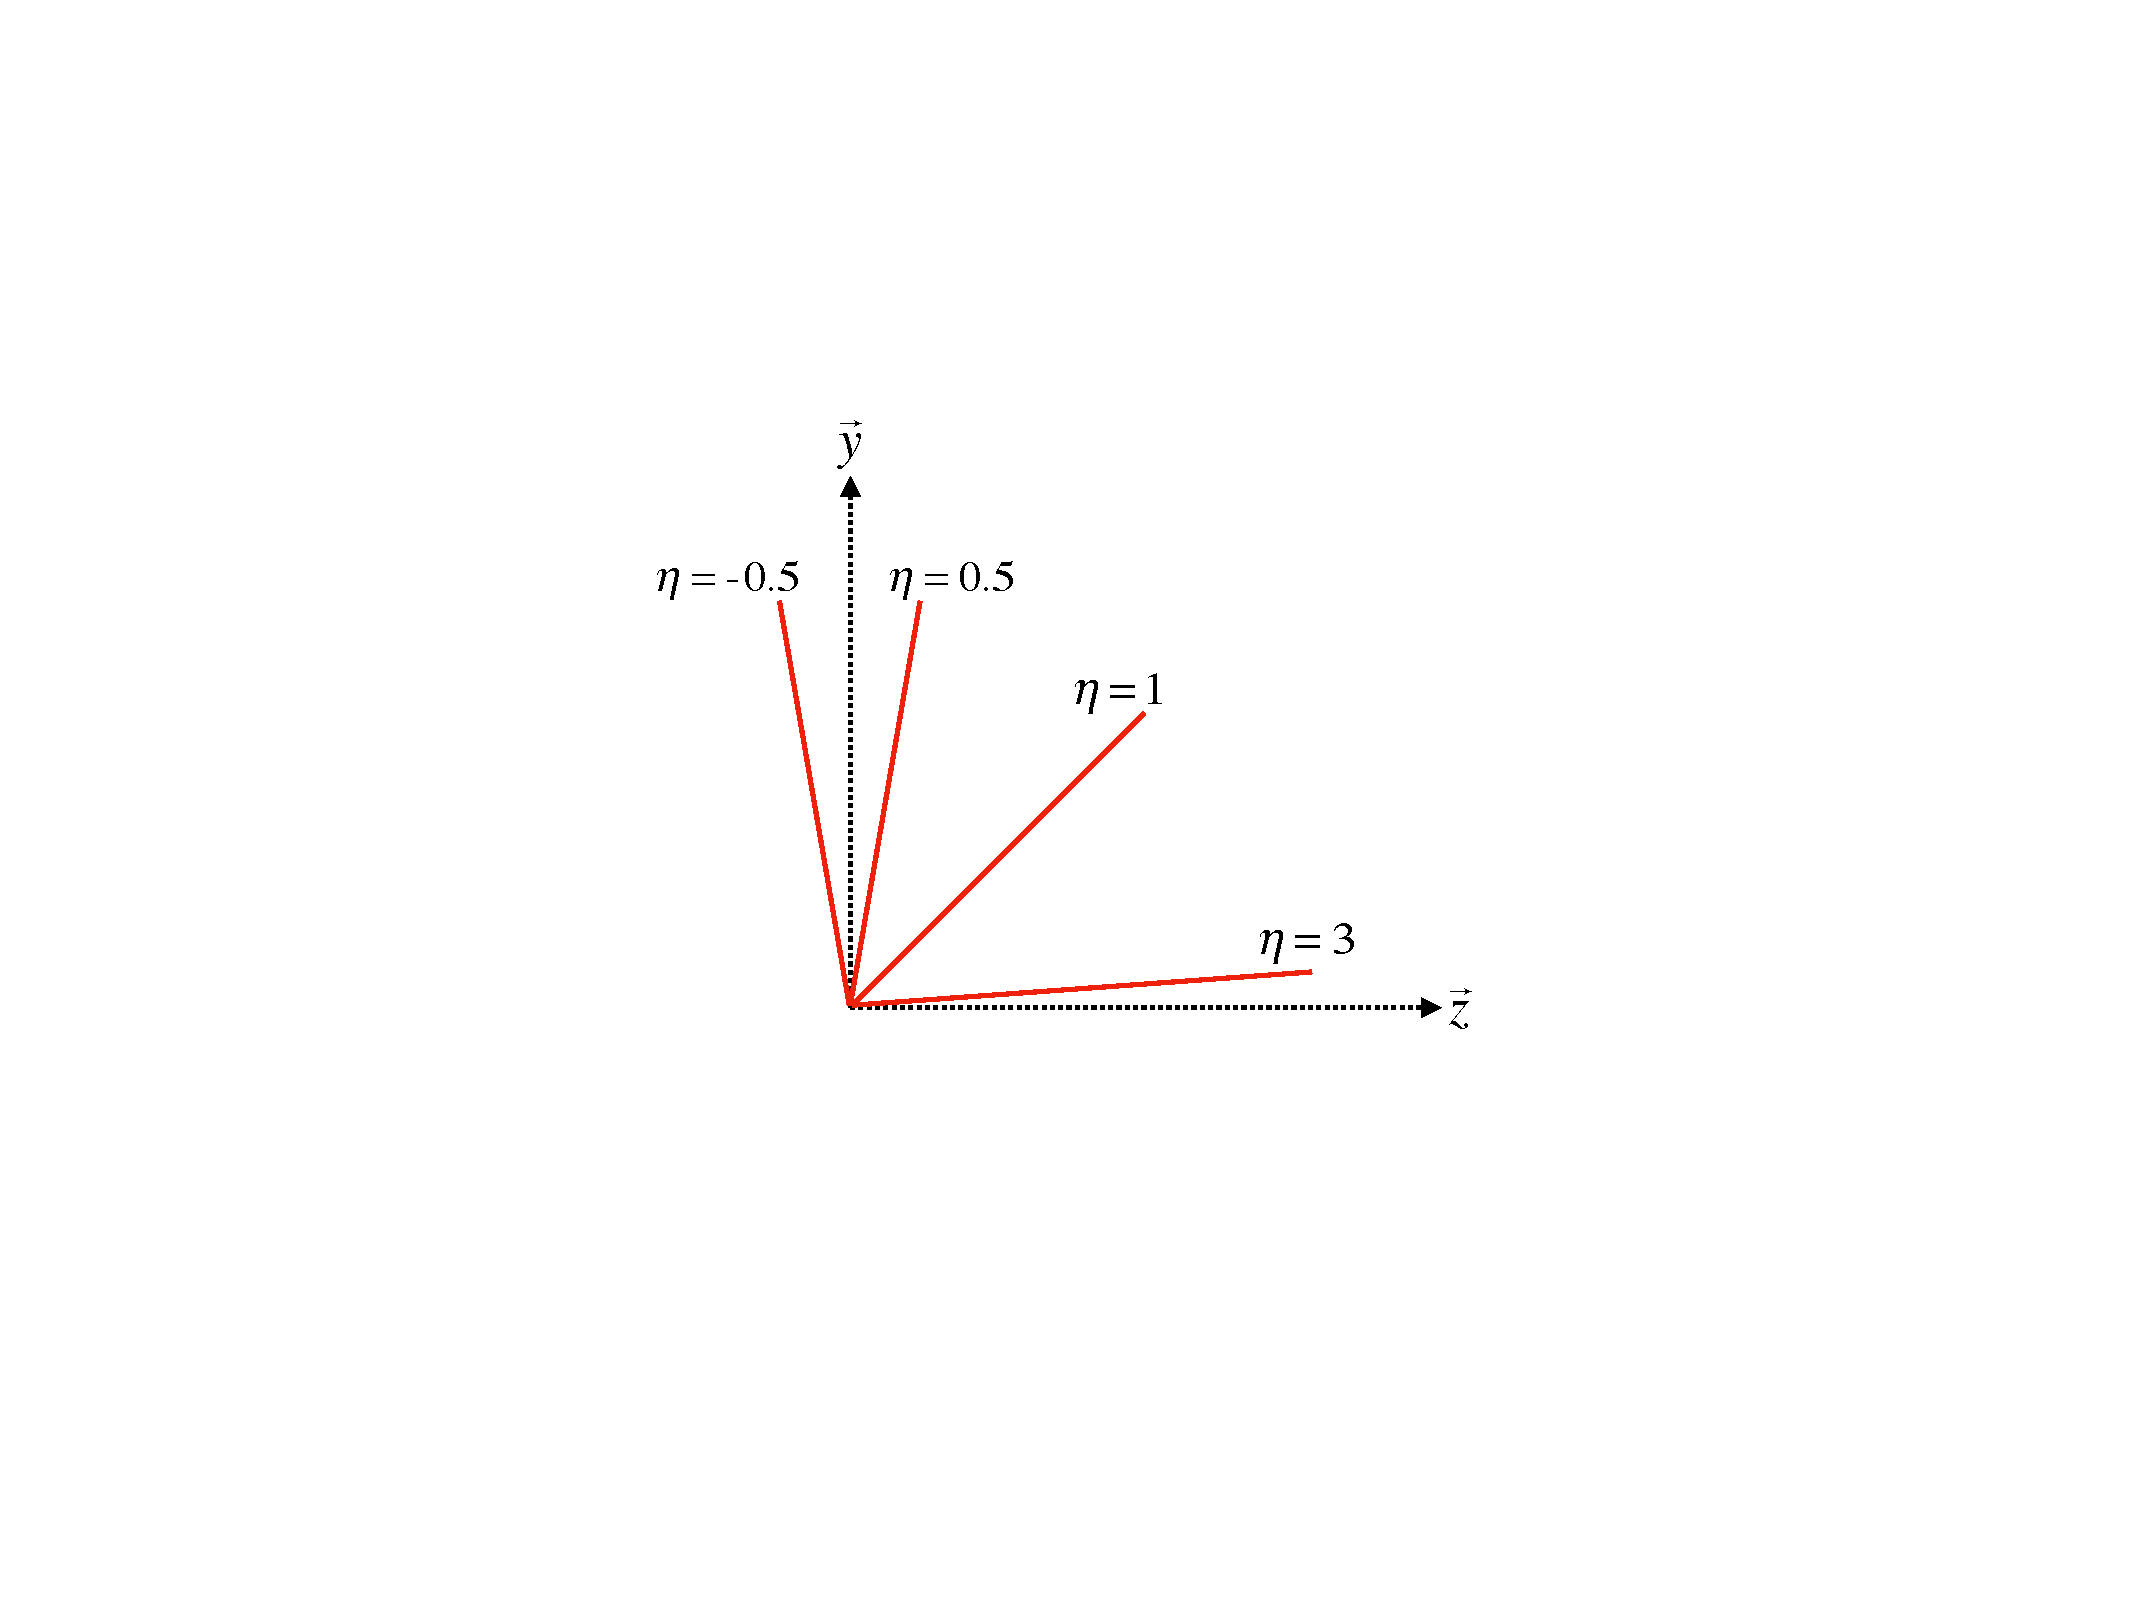
\includegraphics[width=0.5\linewidth]{figures/atlas/pseudorapidity}
    \caption{Modified from \cite{Stark:2317296} this cartoon represents a
selection of pseudorapidity $(\eta)$ values overlaid with some carnelian
coordinates (dashed black lines).  The red lines are drawn for $\eta = \pm
0.5, \; 1.0 and3.0$ }
    \label{fig:pseudorapidity}
  \end{center}
\end{figure}

 
\section{Tracking with the Inner Detector} \label{sec:atlas:tracking}

With its closest component, the Insertable B-Layer (IBL)
\cite{Potamianos:2209070}, only 3.3 cm from the interaction point. The Inner
Detector (ID), shown in \cref{fig:inner_detector_diagram}
\cite{ATLAS-TDR-4,ATLAS-TDR-5}, faces the incredible challenge of providing
precise momentum resolution and identification of both primary and secondary
vertex measurements of charged particle tracks all while receiving the highest fluence.

\begin{figure}[!htbp]
  \begin{center}
    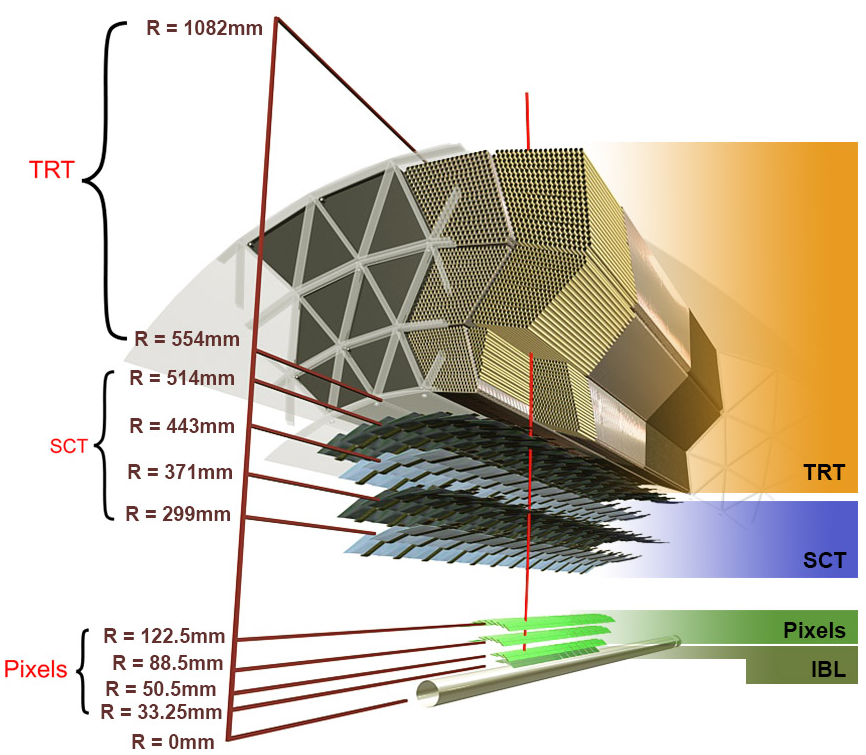
\includegraphics[width=0.8\linewidth]{figures/atlas/inner_detector_diagram}
    \caption{ \cite{Potamianos:2209070} Diagram of inner detector}
    \label{fig:inner_detector_diagram}
  \end{center}
\end{figure}

It is designed to be very compact to reduce the probability of a particle
decaying inside and to give precision measurements of the particles curvature in
the 2T solenoidal magnetic field. This leads to excellent momentum resolution
above the nominal \pT threshold of $0.5$GeV and within the pseudorapidity range
of $|\eta| < 2.5$ as shown in \cref{fig:inner_detector_schematic}.

\begin{figure}[!htbp]
  \begin{center}
    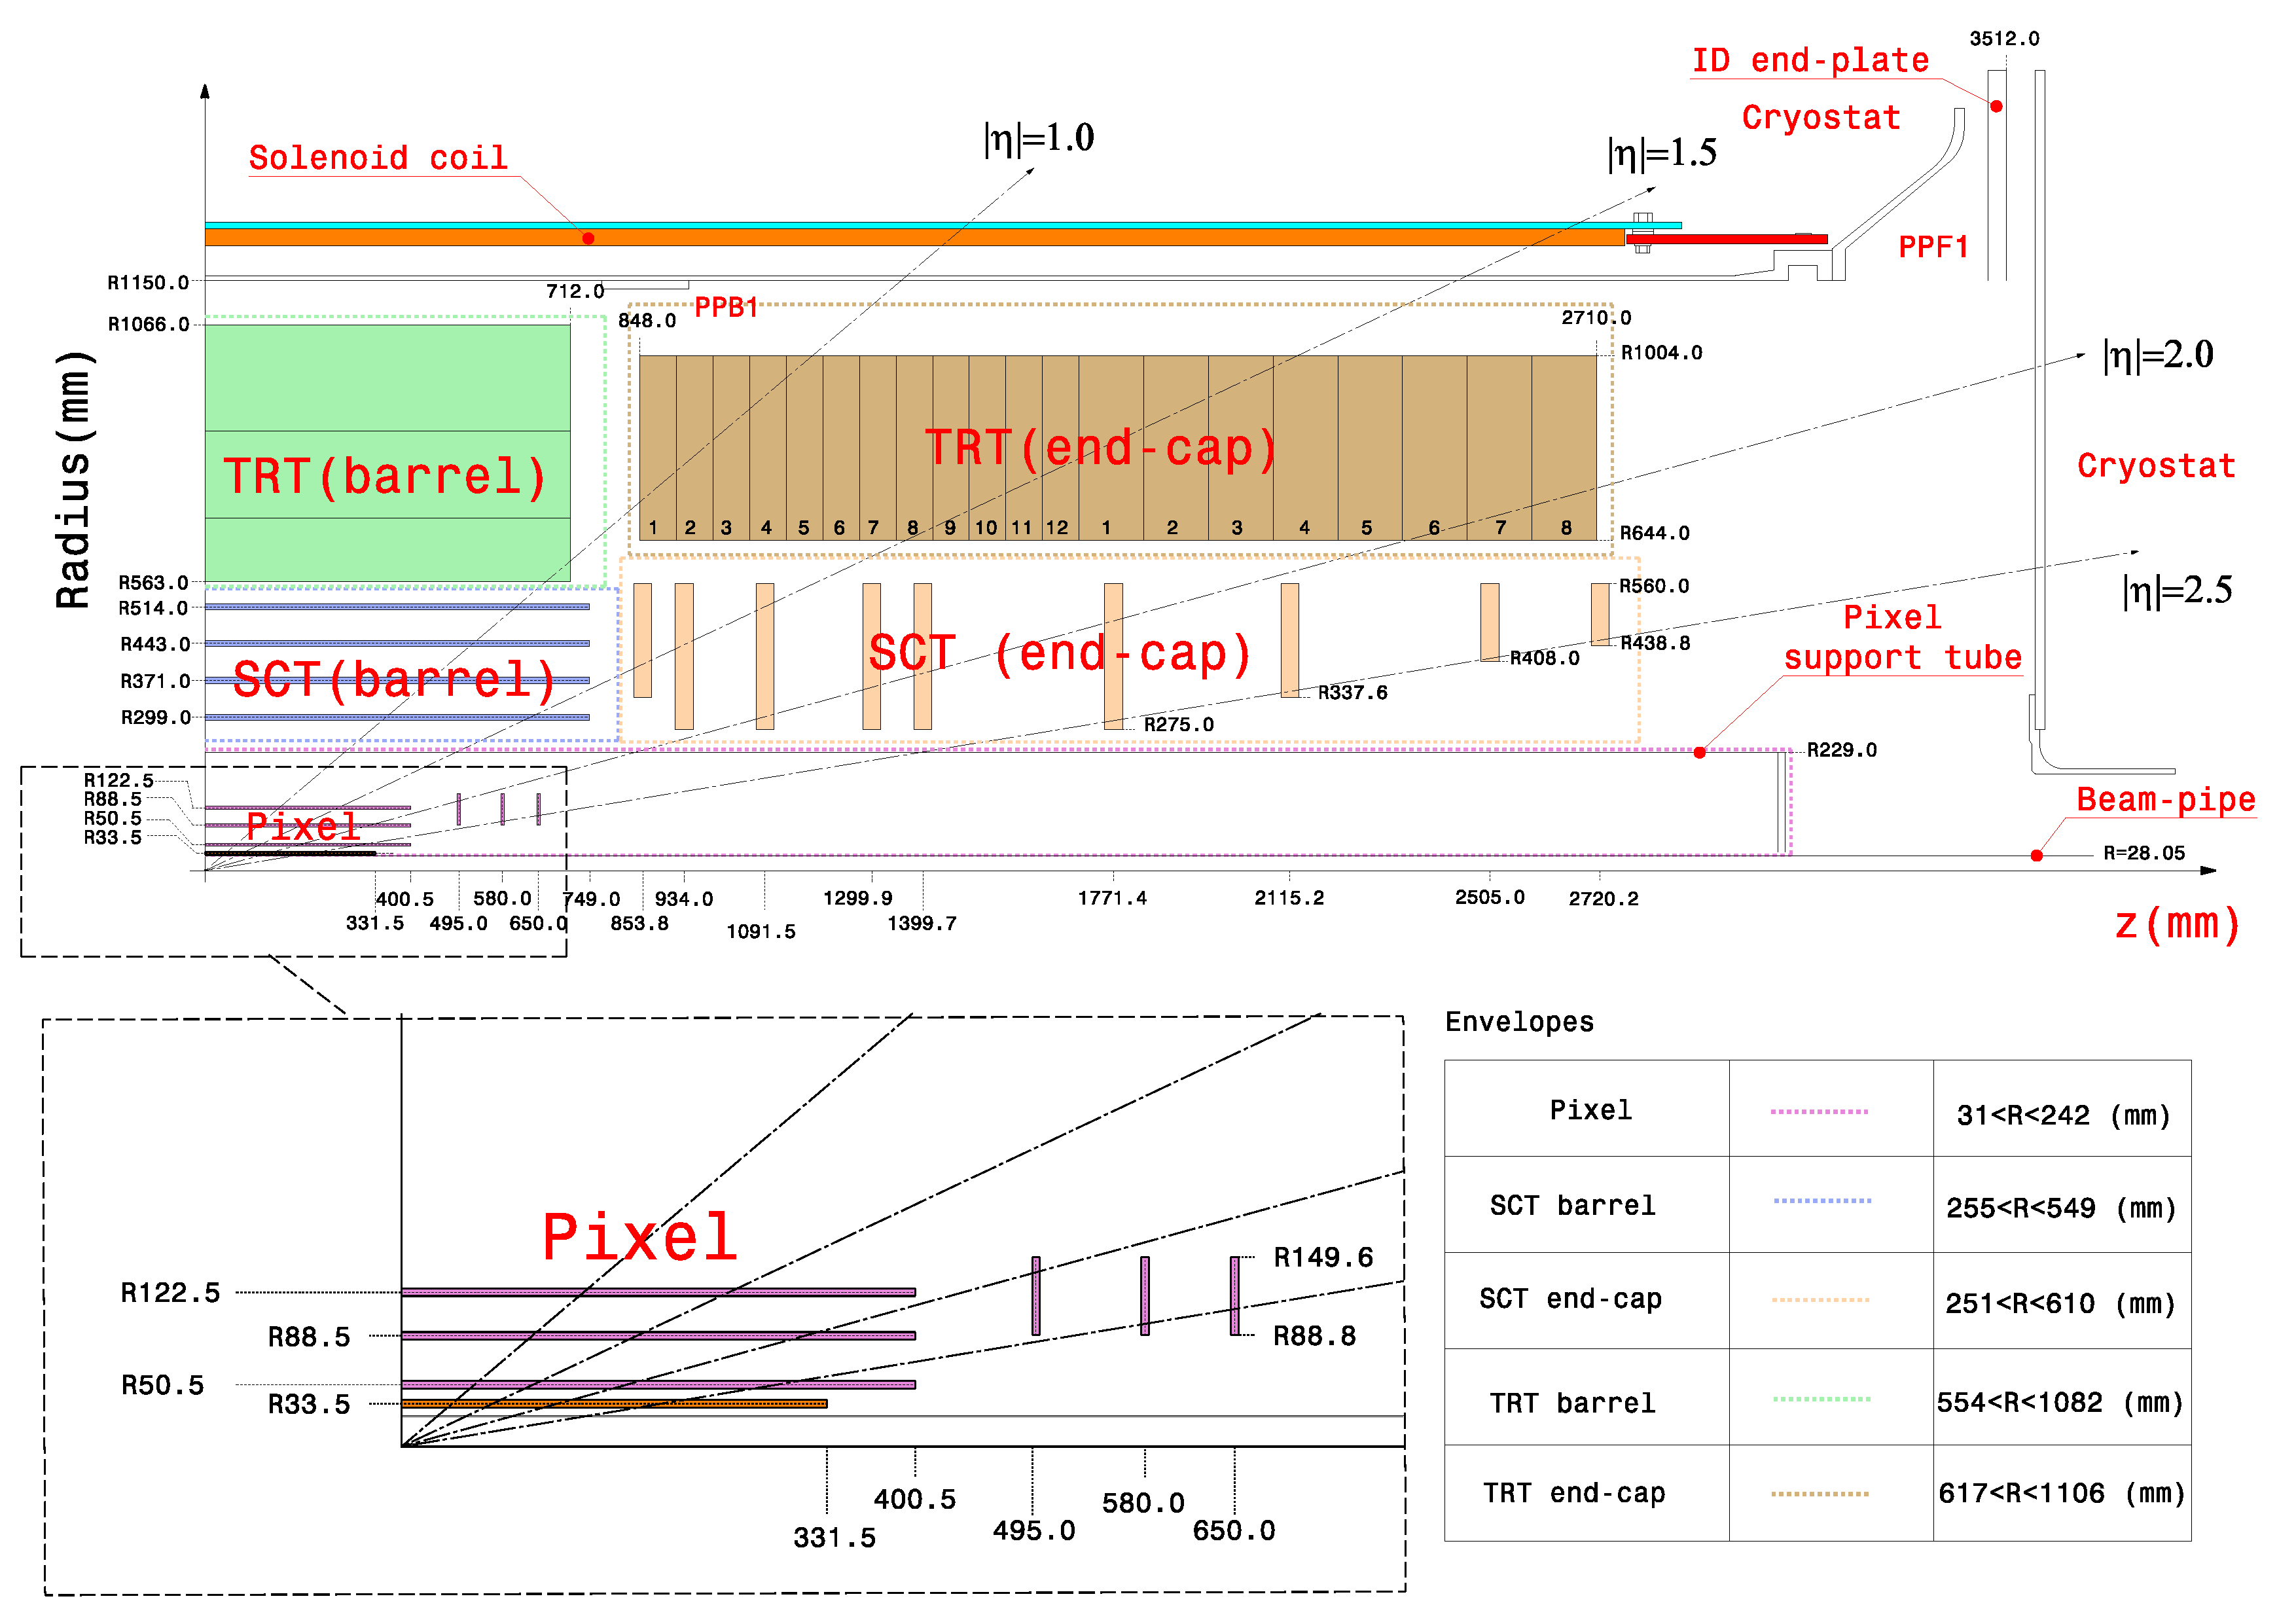
\includegraphics[width=0.8\linewidth]{figures/atlas/inner_detector_schematic}
    \caption{ \cite{PIX-2018-001} Schematic of the Inner Detector including $\eta$
lines.  Each component shown is cylindrically symmetric leading to a
multi-layered detector.}
    \label{fig:inner_detector_schematic}
  \end{center}
\end{figure}

The ID is composed of three different detector technologies for particle
trajector reconstruction: Pixel Detector, Semiconductor Tracker (SCT) and
the Transition Radiation Tracker (TRT).  These will be discussed in the
following sections. 

\subsection{Pixel Detector}

The ATLAS Pixel Detector \cite{PERF-2007-01}, the innermost subdetector of the ID, is designed to
give the best resolution possible as close as possible to the interaction point.
This is accomplished using the 4 barrel layers and 3 disks per endcap as
indicated in \cref{fig:inner_detector_schematic}. The innermost barrel
layer, the IBL, has pixel dimensions of $50\mu $m$(\hat{\phi}) \times 250\mu $m$
(\hat{z}) \times 200\mu $m$(\hat{r})$.  For the other layers the dimensions are
$50\mu $m$(\hat{\phi}) \times 400\mu $m$(\hat{z})$ for about $90\%$ of the pixels
and $50\mu $m$(\hat{\phi}) \times 600\mu $m$(\hat{z})$ for the others, all with a
thickness of $250\mu $m$(\hat{r})$.  This gives a total active area of $1.88 $m$^2$
collected through 92.4 million readout channels, more than half of the total
number of channels for ATLAS. This detailed charged particle information very
close to the interaction point is crucial not only for pattern recognition and
track reconstruction, but also for the reconstruction of the primary and
secondary verticies intrinsic to the decay of $b$-hadrons, a critical element
of the analysis presented in this thesis.

\subsection{Semiconductor Tracker}

Encompassing the Pixel Detector, the Semiconductor Tracker (SCT)
\cite{PERF-2007-01} is composed of double-sided silicon microstrip modules.
Each side of the 4088 modules is constructed out of two silison strip sensors
that are daisy-chained togeather.  The result is 768 composite strips each
$12.6$cm with an inter-strip pitch of $80 \mu$m. In the barrel the strips are
alligned with the $\hat{z}$ direction, while in the end-caps they are aligned
with the $\hat{r}$ direction. In both cases the separation of the strips is
constant in $\hat{\phi}$. The two sides are rotated with respect to each other
by $40 \mu$m to allow for position measurement along the length of the strip.
These modules are then used to tile the 4 barrel layers and 9 disks per endcap
(18 disks in total) as seen in \cref{fig:inner_detector_schematic}.  This
design is chosen to ensure that each charged track interacts with 8 strip
layers (equivalent to four space points).  This information is used to further
measure the momentum and impact parameter, as well as vertex identification of
charged particles.

\subsection{Transition Radiation Tracker}

The Transition Radiation Tracker \cite{PERF-2007-01}, the outermost subdetector
of the ID, provides tracking through the detection of transition radiation from
ultra-relativistic charged particles for $\eta < 2.0$ using 350,000 drift tube
channels also known as straws.  The 4mm diameter straws are filled with a $70\%$
Xe, $27\%$ CO$_2$, and $3\%$ O$_2$ gas mixture and a 31$\mu$m diameter
gold-plated tungsten wire anode at the center for the collection of the
ionization signal. In the barrel 73 azimuthally symetric layers of 144cm straws
are oriented parallel to the beam pipe with an electrical division in the center
of each allowing the two sides to be read out separately.  For each endcap the
straws are radially oriented in 160 symmetric planes each containing 768 37cm
long drift tubes shown in \cref{fig:inner_detector_schematic}.  In both
the barrel and the endcaps polypropylene fibers (barrel) or foils (encaps)
function as the transition radiation material which causes the relativistic
charged particles to radiate and thus ionize the gas in the straw.  The amount
of transition radiation produced is proportional to the Lorentz factor meaning
that lighter particles (e.g. electrons) will produce more radiation.  Thus, by
defining a high and low threshold, we can identify tracks belonging to electrons
by requiring they register more high-threshold hits. There are typically 36 TRT
hits per charged particle track. 
 
\section{Calorimetry} \label{sec:atlas:calorimetry}

\begin{figure}[!htbp]
  \begin{center}
    \includegraphics[width=0.8\linewidth]{figures/atlas/calorimeter_cutaway}
    \caption{ \cite{PERF-2007-01} A cutaway diagram of ATLAS's sampling calorimeters}
    \label{fig:calorimeter_cutaway}
  \end{center}
\end{figure}

Once the proton collision remnants have passed through the ID and it's
surrounding solenoid they enter into the ATLAS calorimeters depicted in figure
\ref{fig:calorimeter_cutaway}.  Sampling calorimeter technologies were choosen
for their compact geometry and lower cost point.  These are constructed by
alternating layers of absorber, a dense material which reduces the incedent
particles energy, and active material which produces a detectible signal when a
partilce passes through.  This means that the detected signal is only a fraction
of the total energy of the particle and thus requires a study of the calorimeter
response for calibration purposes \cite{Fabjan:692252}. The first system, the
Electromagnetic Calorimeter (EMC), is designed to measure the energy of
electrons and photons which primarily lose their energy via bremstralung and
pair production electromagnetic interactions.  Outside of the EMC is the
Hadronic Calorimeter (HC) which is designed to measure the energy of jets of
hadrons through their electromagnetic and strong interactions. These detectors
cover the entire $|\eta| < 4.9$ range and provide complete containment of both
Electromagnetic and Hadronic showers with higher granularityi in the EMC for
$|\eta| < 2.5$, the region matched to the ID, for precision measruements of
electrons and photos.  By instrumenting this huge space in $|\eta|$ we can
search for events with asymetric energy deposits which imply the existence of a
particle we didn't detect represented by missing transverse energy $\MET$.

\subsection{Electromagnetic Calorimeter}

The innermost calorimeter, the Liquid Argon (LAr) Electromagnetic Calorimeter
(EMC) \cite{PERF-2007-01}, uses lead as the absorber and liquid argon as
the active material in an "accordion geometry" as seen in figure
\ref{fig:accordion}. This geometry was choosen for uniform coverage in
$\hat{\phi}$ due to its lack of un-instrumented cracks in the radial direction.
The barrel region covers $|\eta| < 1.475$ and an end cap on each side covers
$1.375 < |\eta| < 3.2$ each housed in their own cryostat.  The barrel is
composed of two half barrels with a 4mm gap at $z = 0$ and both end caps are
divided into an intter wheel covering $2.5 < |\eta| < 3.2$ and an outer wheel
covering $1.375 < |\eta| < 2.5$.

\begin{figure}[!htbp]
  \begin{center}
    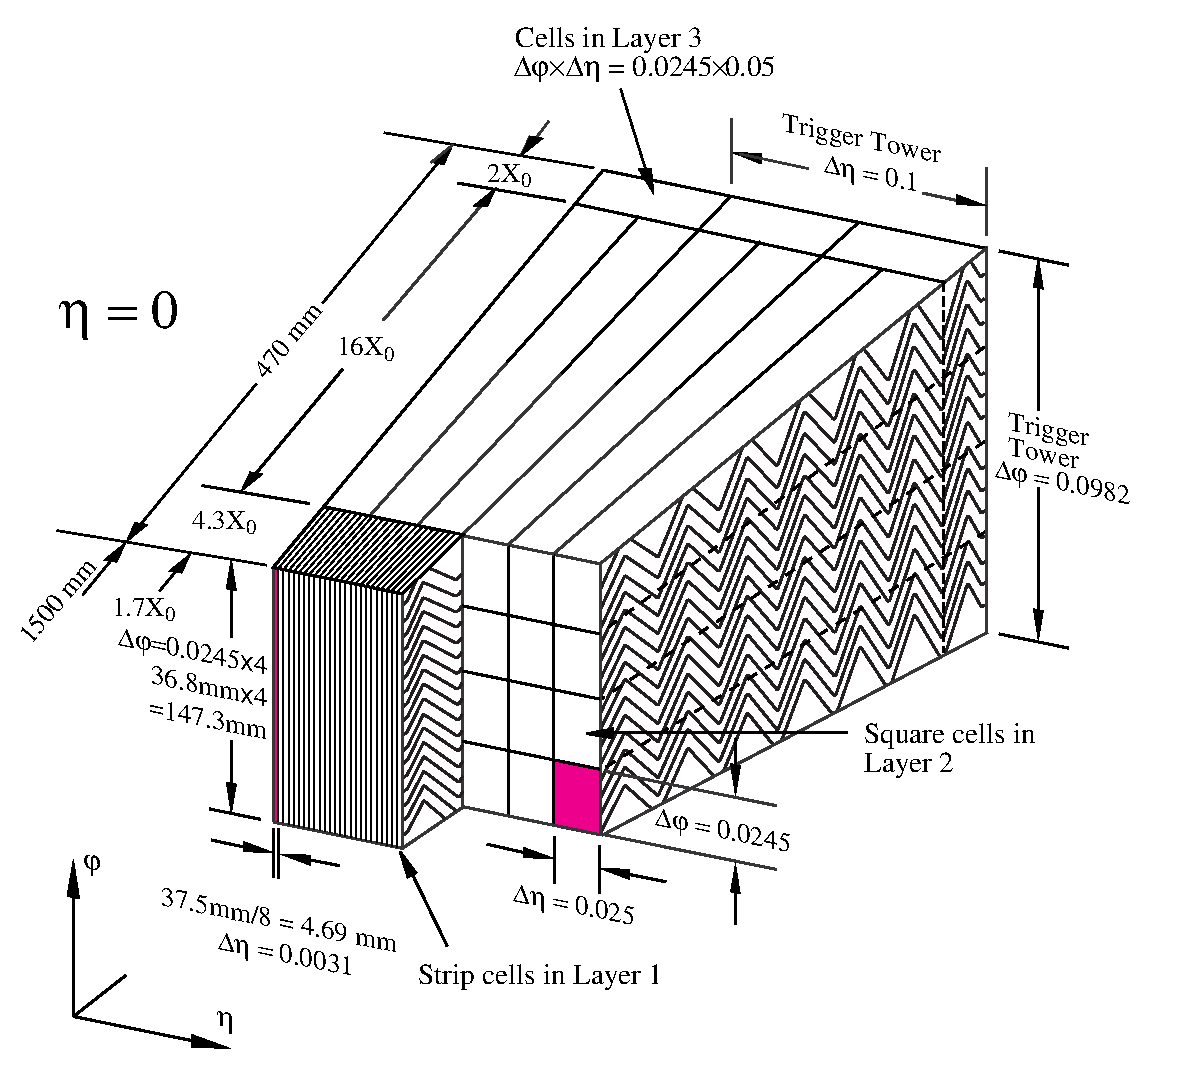
\includegraphics[width=0.8\linewidth]{figures/atlas/accordion}
    \caption{ \cite{PERF-2007-01} Sketch of LAr EMC barrel module where the lead
and liquid argon layers are visible in an accordion like geometry. Looking from
the foreground to the back there are 3 different types of cells visible.}
    \label{fig:accordion}
  \end{center}
\end{figure}

In the $|\eta| < 2.5$ region the EMC has 3 radial layers for precision physics
measurements.  Layer 1 consists of strip cells which are finely segmented with
$\Delta\eta = 0.0031$ and $\Delta\phi = 0.0245$ allowing for precision position
resolution which gives discrimination power between a single $\gamma$ deposit
and the $\pi^0$ characteristic $\gamma\gamma$ deposit. Layer 2 , which collects
the largest fraction of energy from electromagnetic shower, is segmented with
$\Delta\eta = .025$ and $\Delta\phi = 0.0245$. Layer 3 collects the tail of the
electromagnetic shower using a coarser segmentation of $\Delta\eta = .05$ and
$\Delta\phi = 0.0245$.  Additionally, in the region $|\eta| < 1.8$ a thin
pre-sampler , which contains no lead absorber, was placed in front of Layer 1 to
allow for energy corrections due to losses upstream of the EMC.  Combined the
EMC is $>$ 22 radiation lengths ($X_0$) in the barrel and $>$ 24 $X_0$ in the
end-caps, where a radiation length is the average distance an electron travels
in a given material before losing $1/e$ of its original energy $E_0$ via
bremsstrahlung radiation.

\subsection{Hadronic Calorimeter}

Directly outside the EMC envelope is the Hadronic Calorimeter (HC) system
\cite{PERF-2007-01} which consists of three sampling calorimeter technologies:
the Tile calorimeter, the LAr hadronic end-cap calorimeter (HEC) and the LAr
forward calorimeter (FCal).  Combined, these three subsystems give measurements
of hadronic jet energies in the $0 <|\eta| < 4.9$ range. The tile calorimeter
uses steel as the absorber layer and scintillating tiles as the active material
and covers the region $|\eta| < 1.7$ with a barrel section flanked by two barrel
extensions each divided azimuthally into 64 modules.  These scintillator tiles
are read out on two sides by wave-length shifting fibers connected to
photomultiplier tubes as seen in figure \ref{fig:tile_calorimeter}. At $\eta =
0$ the total tile calorimeter thickness is 9.7 nuclear interaction lengths
($\lambda$), where $\lambda$ is the average distance a hadron travels before
interacting inellastically with a nucleus.

\begin{figure}[!htbp]
  \begin{center}
    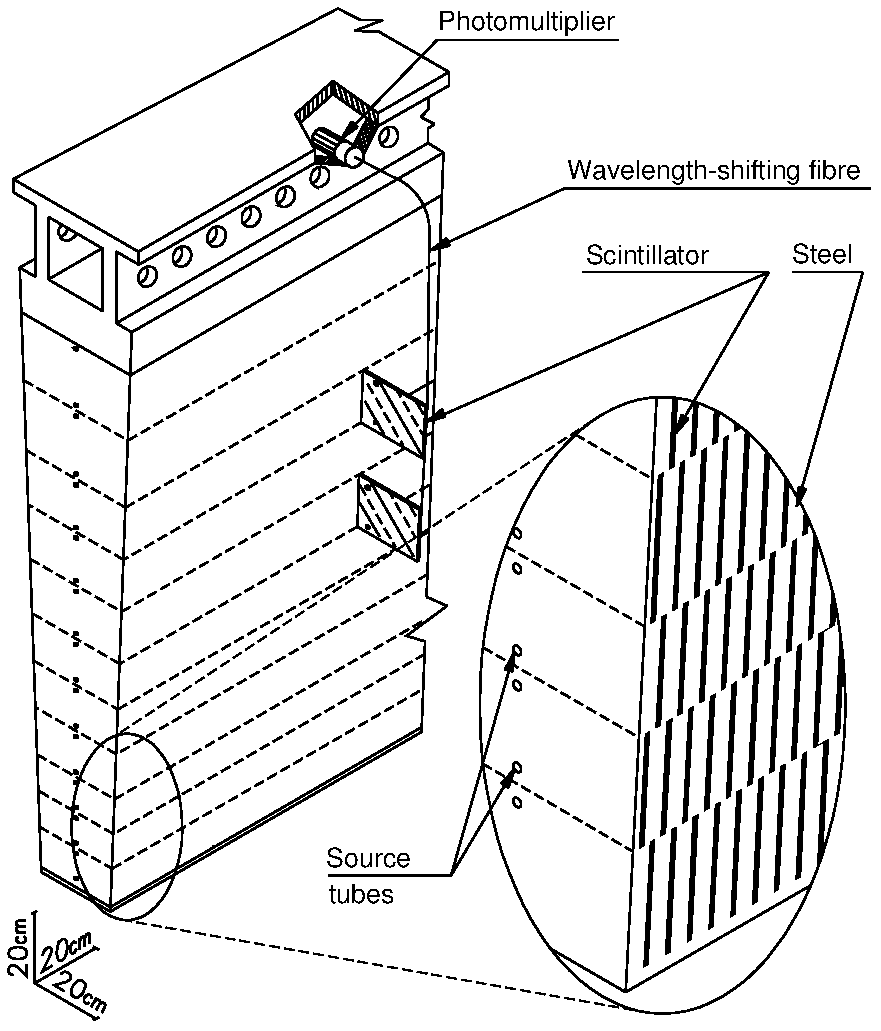
\includegraphics[width=0.8\linewidth]{figures/atlas/tile_calorimeter.pdf}
    \caption{ \cite{PERF-2007-01} Schematic of a tile calorimeter module
including a depiction of the connection between the scintillator tile to the
photomultiplier via a wavelength-shifting fibre.}
    \label{fig:tile_calorimeter}
  \end{center}
\end{figure}

The HEC is composed of two independent wheels per end-cap located just past the
EMC end-cap but sharing the same cryostat. This system  uses copper as an
absorber and liquid argon for the active material and covers the $1.5 < |\eta| <
3.2$ range using 32 wdge-shaped modules per wheel. Finally, the FCal shares the
same cryostat as the EMC and HEC end-caps and acts to extend the coverage of the
combined calorimeter system to include the $3.1 < |\eta| < 4.9$ range.  Each
endcap contains 3 modules, the first an electromagnetic module
(Copper/Liquid-Argon) which is followed by two hadronic modules which use
(Tungsten/Liquid-Argon.

\section{Muon Spectrometer} \label{sec:atlas:muons}

The ATLAS Muon Spectrometer (MS) \cite{PERF-2007-01}, see
\Cref{fig:muon_system}, accomplishes tracking of muons in the $|\eta| < 2.7$
region for momentum reconstruction while also triggering on charged particles
in the $|\eta| < 2.4$ region.  The magnetic field necessary for momentum
reconstruction is provided by 3 air-core toroid systems, one barrel toroid
covering $|\eta| < 1.4$ and two end-cap toroid systems which are inserted into
the inner radius of the barrel toroid to cover the $1.6 < |\eta| < 2.7$. The
so-called transition region $1.4 < |\eta| < 1.6$ between these two magnet
systems is covered by a combination of the barrel and end-cap toroid magnets.
Similar to the ID the resolution in the MS is inversely proportional to the particle's
incident momentum.  Any muon with $\pt$ lower than $\sim 3~\GeV$ will never
make it to the MS due to energy loss in the calorimeters \cite{PERF-2007-01}.

\begin{figure}[!htbp]
  \begin{center}
    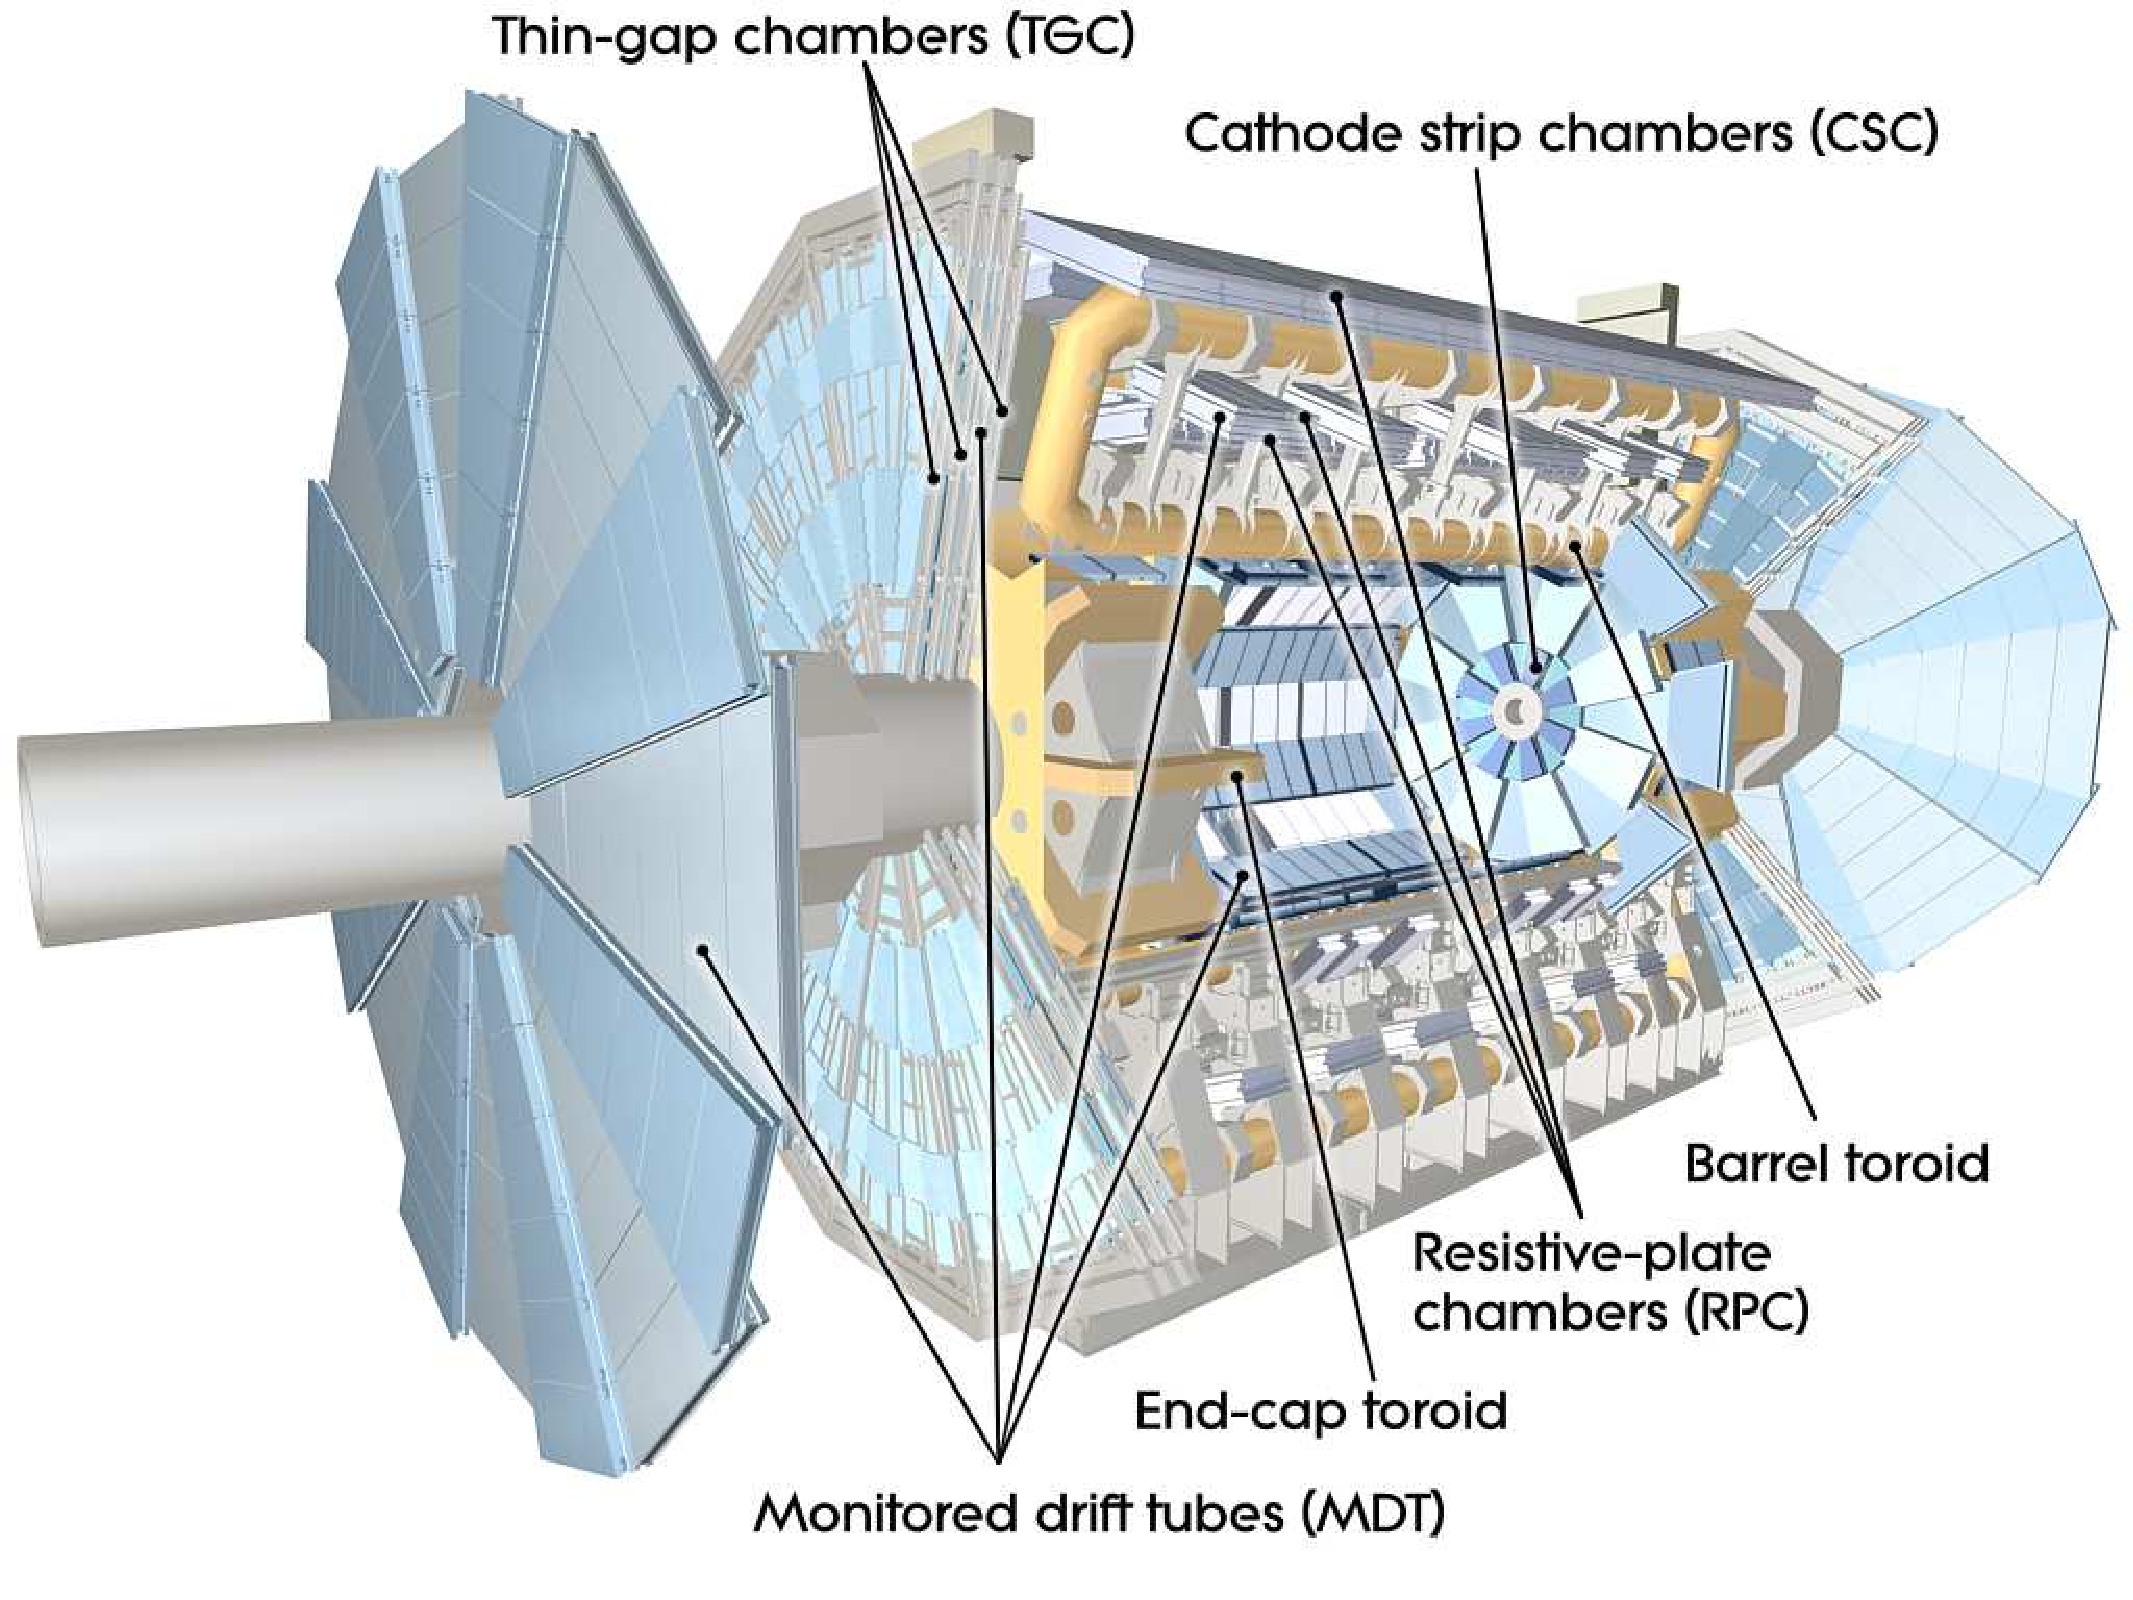
\includegraphics[width=0.8\linewidth]{figures/atlas/muon_system}
    \caption{A cut-away diagram of the ATLAS muon system
and its many sub-detectors \cite{PERF-2007-01}.}
    \label{fig:muon_system}
  \end{center}
\end{figure}

Precision tracking measurements for momentum reconstruction is accomplished
using the Monitored Drift Tube chambers (MDTs) for $|\eta| < 2.0$.  The MDT
system consists of 1163 drift tube chambers arranged in three to eight layers
for varying $\eta$.  The Cathode-Strip Chambers (CSCs) span the range $2.0 <
|\eta| < 2.7$ and are designed to withstand the higher rate at high $\eta$ and
retain good time resolution using multiwire proportional chambers with
orthogonal segmented cathode planes.

The MS also gives nanosecond tracking information for triggering on muon tracks.
This is accomplished using Resistive Plate Chambers (RPC) in the barrel region
$|\eta| < 1.05$ and Thin Gap Chambers (TGC) in the end-cap $1.05 < |\eta| < 2.4$
region.  Both chamber systems deliver a triggerable signal with a spread of
$15-25$ ns, thus providing the ability to tag individual beam-crossings.

